\begin{figure}[htb]
\centering
\includegraphics[page=4,width=0.25\textwidth]{\FCNCFigures/r21/thq2tau/SSOSWithFakeMCCalibrated/reg2mtau1b2jos/BDTG_test.pdf}
\put(-30, 80){\textbf{(a1)}}
\includegraphics[page=5,width=0.25\textwidth]{\FCNCFigures/r21/thq2tau/SSOSWithFakeMCCalibrated/reg2mtau1b2jos/BDTG_test.pdf}
\put(-30, 80){\textbf{(a2)}}
\includegraphics[width=0.25\textwidth]{\FCNCFigures/r21/thq2tau/ROC/reg2mtau1b2jos.pdf}
\put(-70, 70){\textbf{(a3)}}\\
\includegraphics[page=4,width=0.25\textwidth]{\FCNCFigures/r21/thq2tau/SSOSWithFakeMCCalibrated/reg2mtau1b3jos/BDTG_test.pdf}
\put(-30, 80){\textbf{(b1)}}
\includegraphics[page=5,width=0.25\textwidth]{\FCNCFigures/r21/thq2tau/SSOSWithFakeMCCalibrated/reg2mtau1b3jos/BDTG_test.pdf}
\put(-30, 80){\textbf{(b2)}}
\includegraphics[width=0.25\textwidth]{\FCNCFigures/r21/thq2tau/ROC/reg2mtau1b3jos.pdf}
\put(-70, 70){\textbf{(b3)}}\\
\includegraphics[page=4,width=0.25\textwidth]{\FCNCFigures/tthML/showFake/faketau/postfit/NOMINAL/reg1l1tau1b2j_os/BDTG_test.pdf}
\put(-30, 80){\textbf{(c1)}}
\includegraphics[page=5,width=0.25\textwidth]{\FCNCFigures/tthML/showFake/faketau/postfit/NOMINAL/reg1l1tau1b2j_os/BDTG_test.pdf}
\put(-30, 80){\textbf{(c2)}}
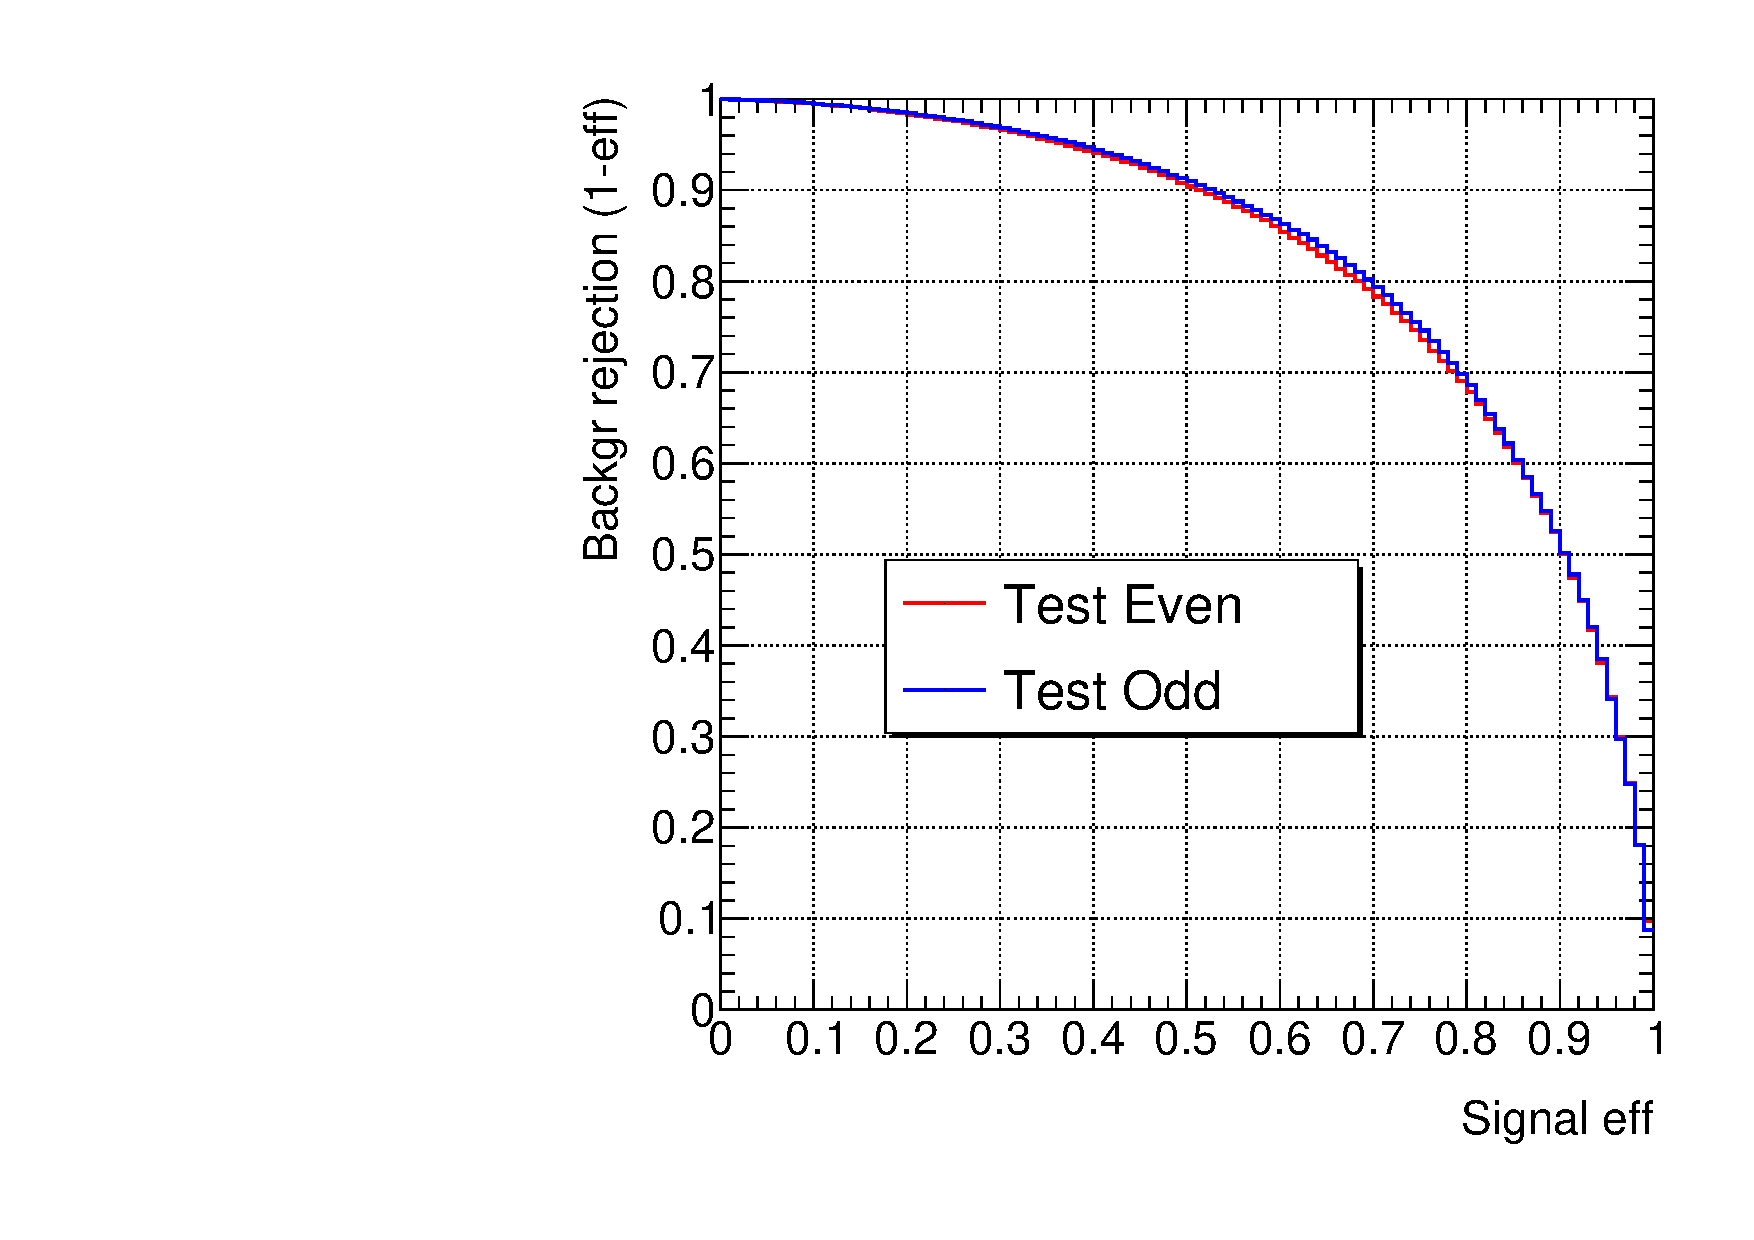
\includegraphics[width=0.25\textwidth]{\FCNCFigures/tthML/BDT/roc_reg1l1tau1b2j_os.pdf}
\put(-70, 70){\textbf{(c3)}}\\
\includegraphics[page=4,width=0.25\textwidth]{\FCNCFigures/tthML/showFake/faketau/postfit/NOMINAL/reg1l1tau1b3j_os/BDTG_test.pdf}
\put(-30, 80){\textbf{(d1)}}
\includegraphics[page=5,width=0.25\textwidth]{\FCNCFigures/tthML/showFake/faketau/postfit/NOMINAL/reg1l1tau1b3j_os/BDTG_test.pdf}
\put(-30, 80){\textbf{(d2)}}
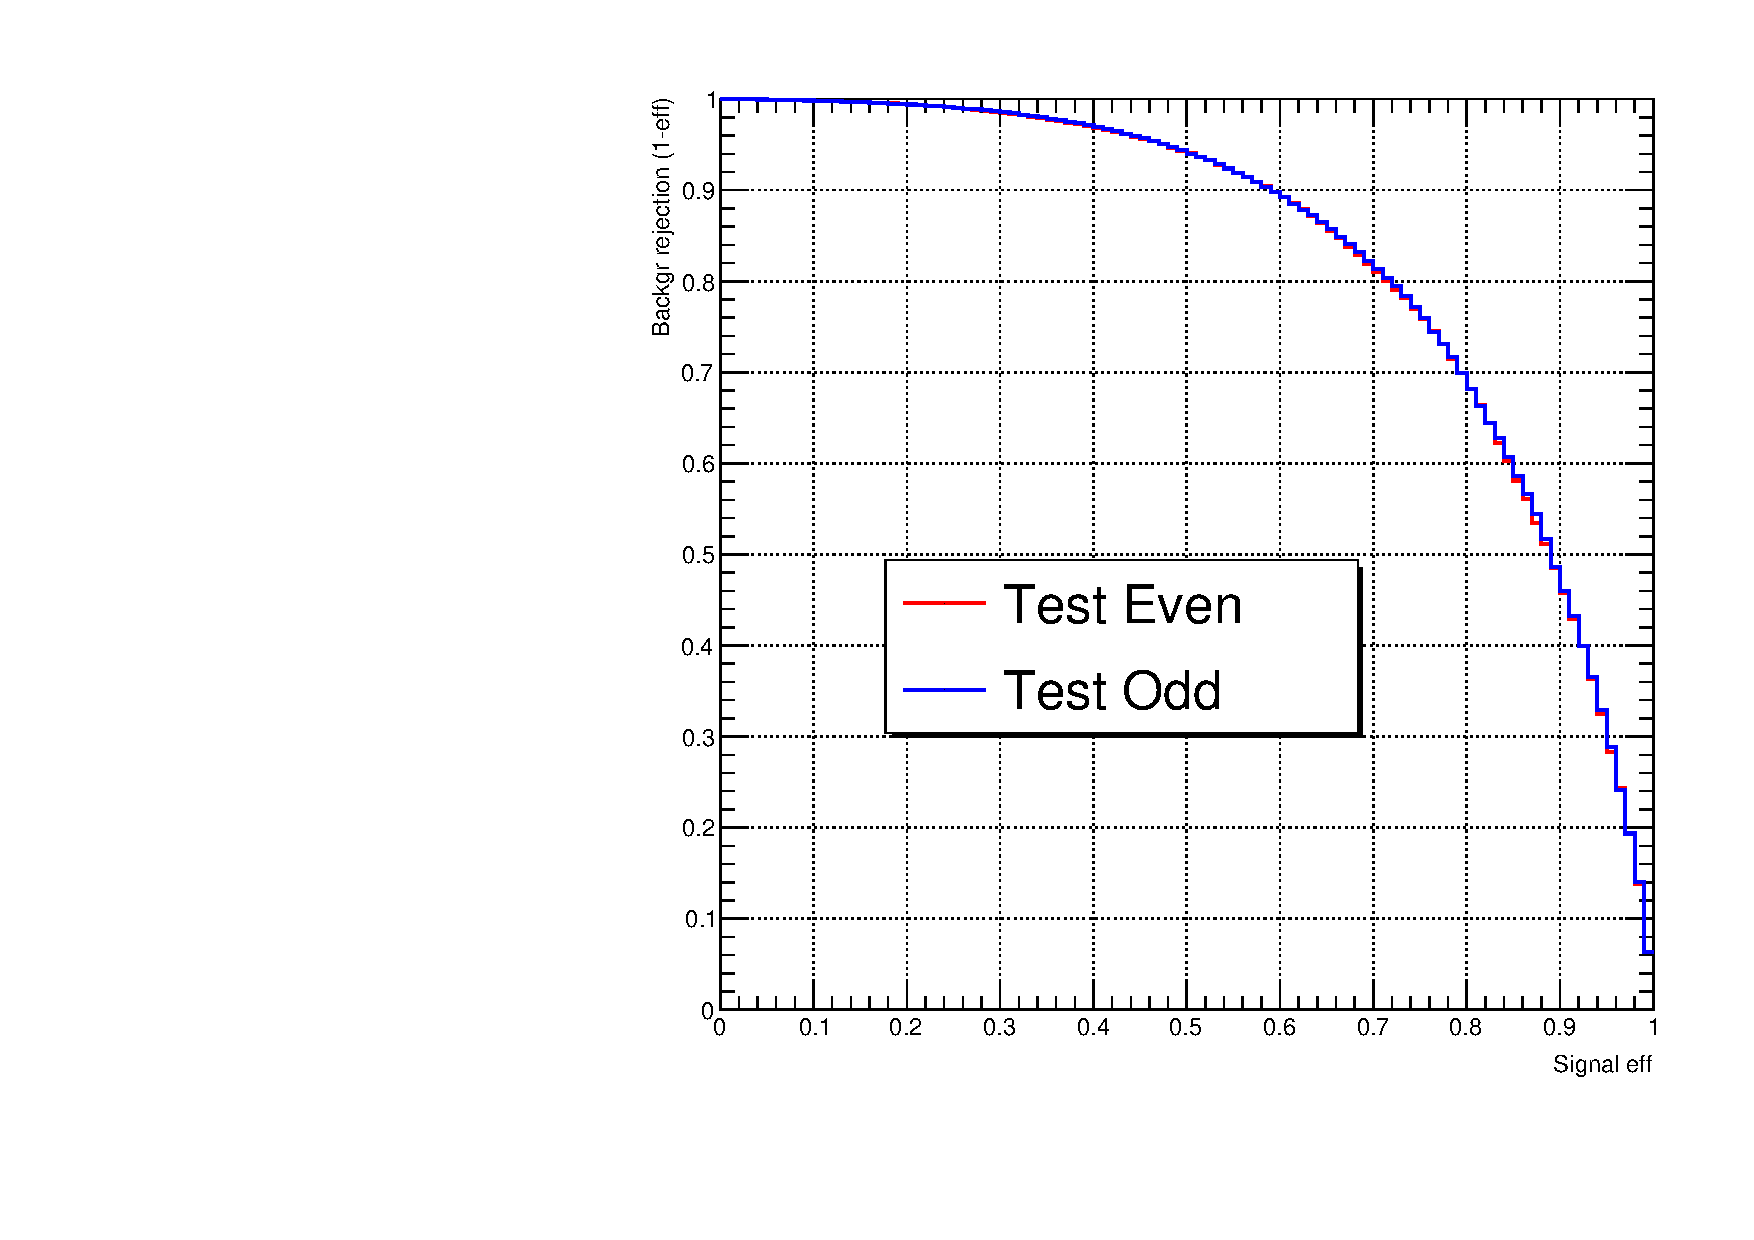
\includegraphics[width=0.25\textwidth]{\FCNCFigures/tthML/BDT/roc_reg1l1tau1b3j_os.pdf}
\put(-70, 70){\textbf{(d3)}}\\
\includegraphics[page=4,width=0.25\textwidth]{\FCNCFigures/tthML/showFake/faketau/postfit/NOMINAL/reg1l2tau1bnj_os/BDTG_test.pdf}
\put(-30, 80){\textbf{(e1)}}
\includegraphics[page=5,width=0.25\textwidth]{\FCNCFigures/tthML/showFake/faketau/postfit/NOMINAL/reg1l2tau1bnj_os/BDTG_test.pdf}
\put(-30, 80){\textbf{(e2)}}
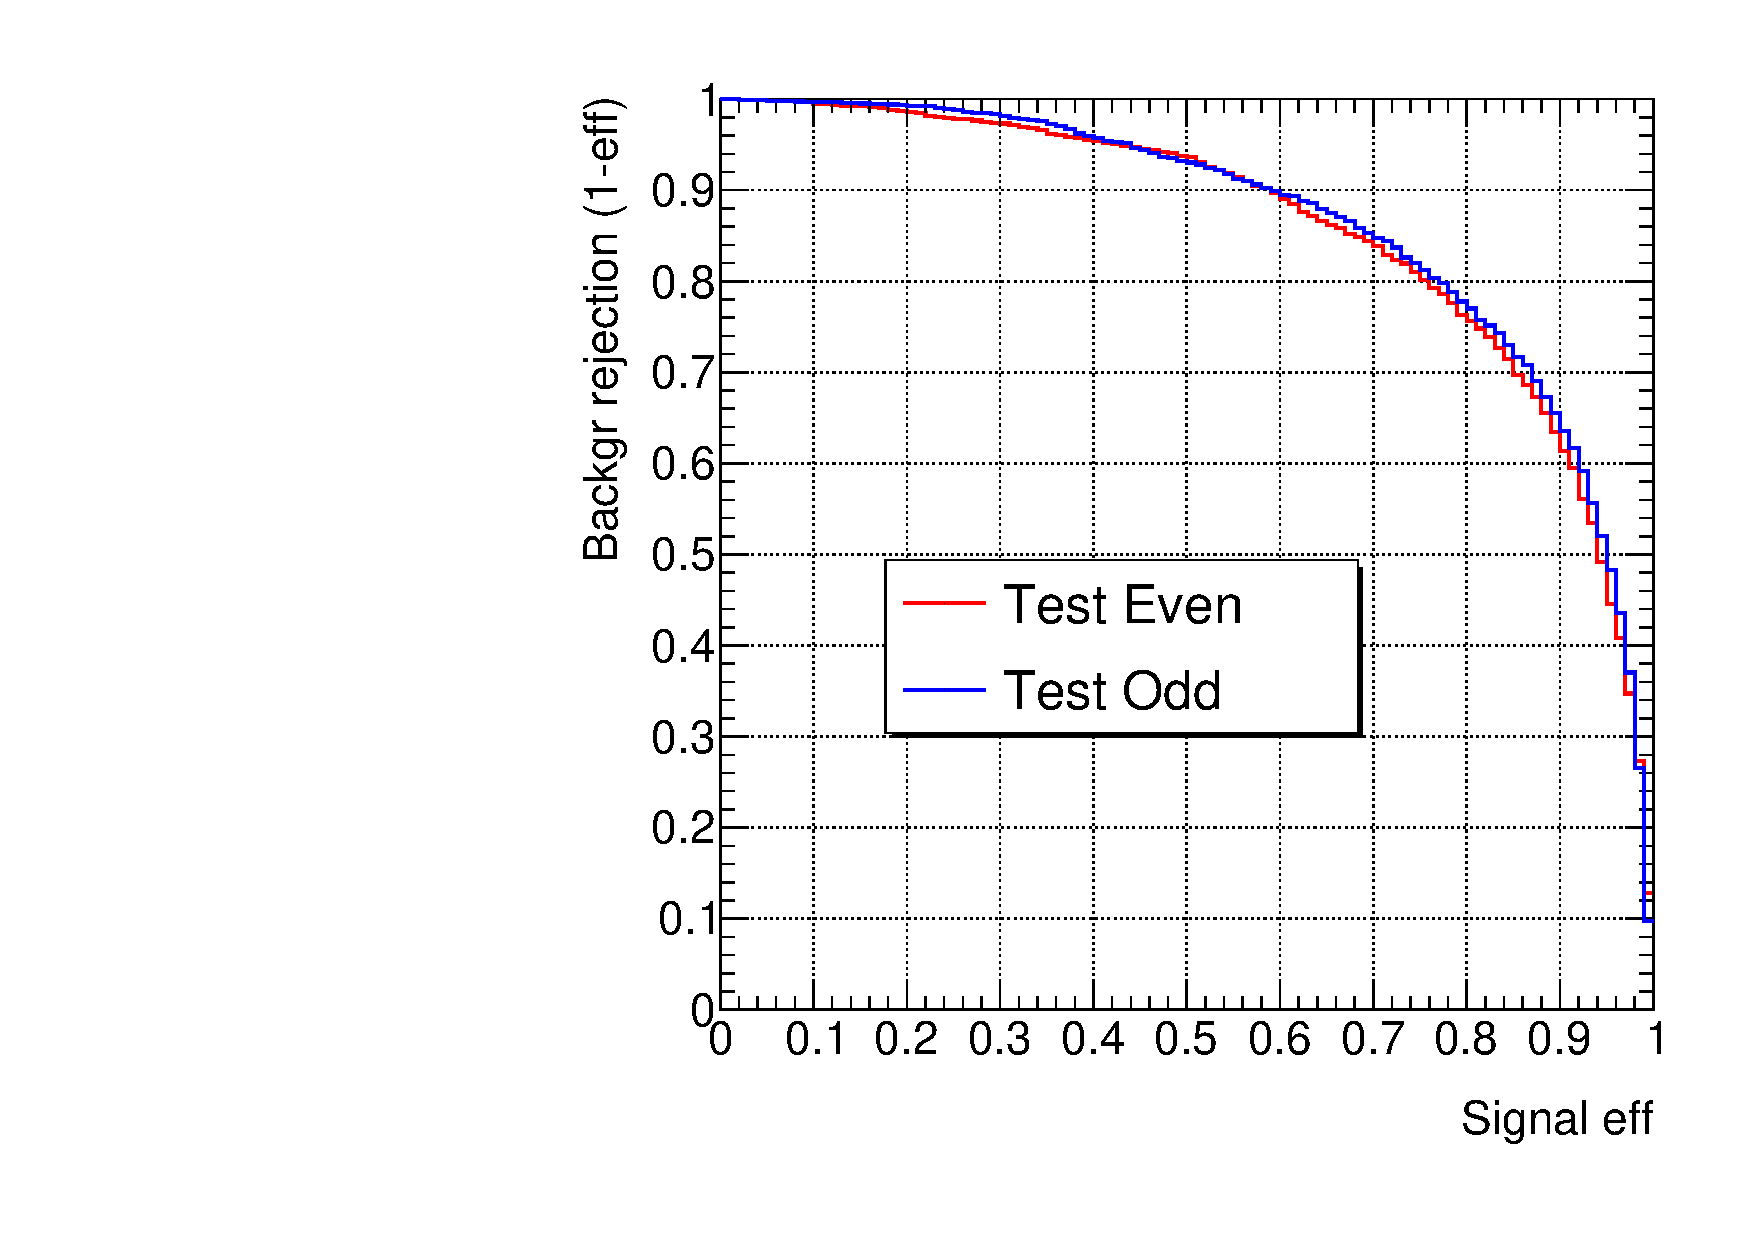
\includegraphics[width=0.25\textwidth]{\FCNCFigures/tthML/BDT/roc_reg1l2tau1bnj_os.pdf}
\put(-70, 70){\textbf{(e3)}}\\
\caption{ The BDT output distributions for the background and TT signal (a1, b1, c1, d1, e1), background and ST signal (a2, b2, c2, d2, e2) and ROC curves (a3, b3, c3, d3, e3) in the STH $\thadhad$ (a1-3), TTH $\thadhad$ (b1-3), STH $\tlhad$ (c1-3), TTH $\tlhad$ (d1-3),  $l\thadhad$ (e1-3) channels. }% The Kolmogorov Test values for the training and testing BDT distributions are also indicated.
\label{fig:overtrain}
\end{figure}
